\documentclass{ctexart}
\title{序列模型}
\author{姚兴虎}
\date{\today}

\usepackage{geometry}
\geometry{a4paper,scale=0.8}
\usepackage{amsfonts}
\usepackage{amsmath}
\usepackage{amssymb}
\usepackage{graphicx}
\usepackage{subfig}
\usepackage{dsfont}
\newtheorem{Def}{\hspace{2em}定义}
\newtheorem{Theo}{\hspace{2em}定理}
\begin{document}
\maketitle
\section{循环序列模型}
\subsection{序列数据的例子}
现实世界中的许多数据都可以用序列数据来表示,比如:语音识别问题中的输入数据是一个语音片段,输出是一个文字序列;音乐生成问题的输出数据是一段音乐;情感分类的输入数据是一个或多个句子;DNA序列分析中的输入数据是DNA序列等。这些问题都可以认为是给定输入数据和数据标签的监督学习问题,其中输入数据$X$或数据标签$Y$以序列数据的形式来表示。
\subsection{数学符号}
我们考虑这样一个例子:我们的输入数据是一个句子,我们希望识别出这个句子中的每个单词是不是人名,若句子中的当前单词是人名,则对应位置的输出为1,否则为0。如下所示:$x:$  Harry Potter and Hermione Granger invented a new spell.我们知道,Harry Potter 和 Hermione是人名,而其它的词汇不是人名,因此我们期望得到的输出向量$y=[1,1,0,1,1,0,0,0]^T$。对于这个输入和输出序列,我们用$T_X$来表示输入序列的长度,$T_y$来表示输出序列的长度,在这里我们有:$T_x = T_y =9$。注意输入和输出序列的长度并不总是相等的。我们用$x^{<t>}$来表示序列中的第$t$个数据,在这里:$x^{<1>}=Harry,x^{<3>}=and$我们的数据集中通常含有大量的数据,假设训练集中输入序列的集合为$X$,则$X^{(i)},Y^{(i)},T_x^{<i>},T_y^{<i>}$分别表示数据集中第$i$个样本的输入,输出,输入长度,输出长度。用$X^{(i)<t>},Y^{(i)<t>}$来表示第$i$个样本的第$t$个位置的数据。在将数据输入到模型中进行拟合时,我们还需要对这种非数值的序列化数据进行表示,通常的表示方法包括one-hot表示和词嵌入(word embedding)表示,在这里我们不再展开叙述。
\subsection{循环神经网络模型}
在介绍循环神经网络之前,我们先考虑为什么不能利用传统的神经网络结构来处理序列化的数据呢,如下图所示:输入数据是一个句子,经过全连接网络得到其输入。
\begin{figure}[ht]
\centering
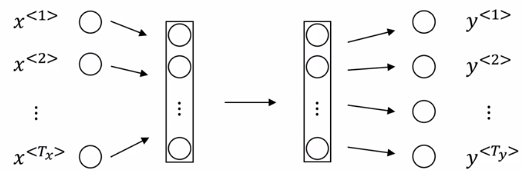
\includegraphics[scale=0.6]{1.png}
\end{figure}


事实上,这一方法存在的两个大问题使得这种传统的结构难以用来处理序列数据。
(1)不同样本的输入和输出往往具有不同的长度,我们可以对数据进行0填充或者1填充来使得数据之间的维度相适应,但这破坏了数据的原始结构,不是一个好的方法。(2)这样简单的网络结构不能够共享从数据的不同位置所得到的特征。比方说,当出现Harry时后面紧接着出现的单词很可能是一个人名,我们希望网络将这种学习到的信息进行共享,而这与卷积神经网络中的将图片中学习到的特征表示利用到其他图像类似。此外,通过权重共享也能够减少网络参数的规模。我们将要介绍的循环神经网络便能够克服这两个缺点。


一个简单的循环神经网络的前向传播过程如下所图所示:我们首先可以将第一个$a^{<0>}$初始化为零向量,然后进行前向传播过程,$a^{<1>}=g(W_{aa}a^{<0>}+b_a),\hat{y}^{<1>}=g(W_{ya}a^{<1>}+b_y)$,其中$W_{ax}$是将$x$变换成$a$的一个参数矩阵。隐藏层的激活函数通常选取tanh,但是有时也选取relu。输出层的激活函数根据不同的问题可选取不同类型的激活函数,例如分类问题中常常选取sigmoid或者softmax。

\begin{figure}[ht]
	\centering
	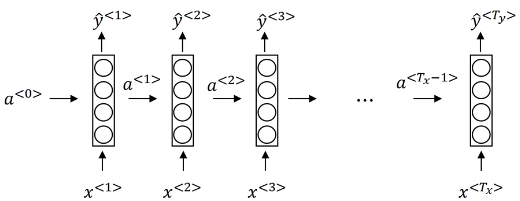
\includegraphics[scale=0.6]{2.png}
\end{figure}
在一般情形下,上述符号可以写为:
\begin{align*}
a^{<t>} &= g(W_{aa}a^{<t>}+W_{ax}x^{<t>}+b_a)\\
\hat{y}^{<t>}&=g(W_{ya}a^{<t>}+b_y)
\end{align*}
还可以将$W_{aa}$与$W_{ax}$合并从而得到更为精简的前向计算公式:
\begin{align*}
a^{<t>} &= g(W_{a}[a^{<t>},x^{<t>}]+b_a)\\
\hat{y}^{<t>}&=g(W_{y}a^{<t>}+b_y).
\end{align*}


一个基本的RNN模块如下图所示,该模块的输入是当前的输入$x^{<t>}$和由过去所有的隐藏状态累计下来的信息$a^{<t-1>}$,模块的输出是传入到下一个时刻的隐藏信息$a^{<t>}$和当前的预测信息$\hat{y}^{<t>}$。
\begin{figure}[htb!]
	\centering
	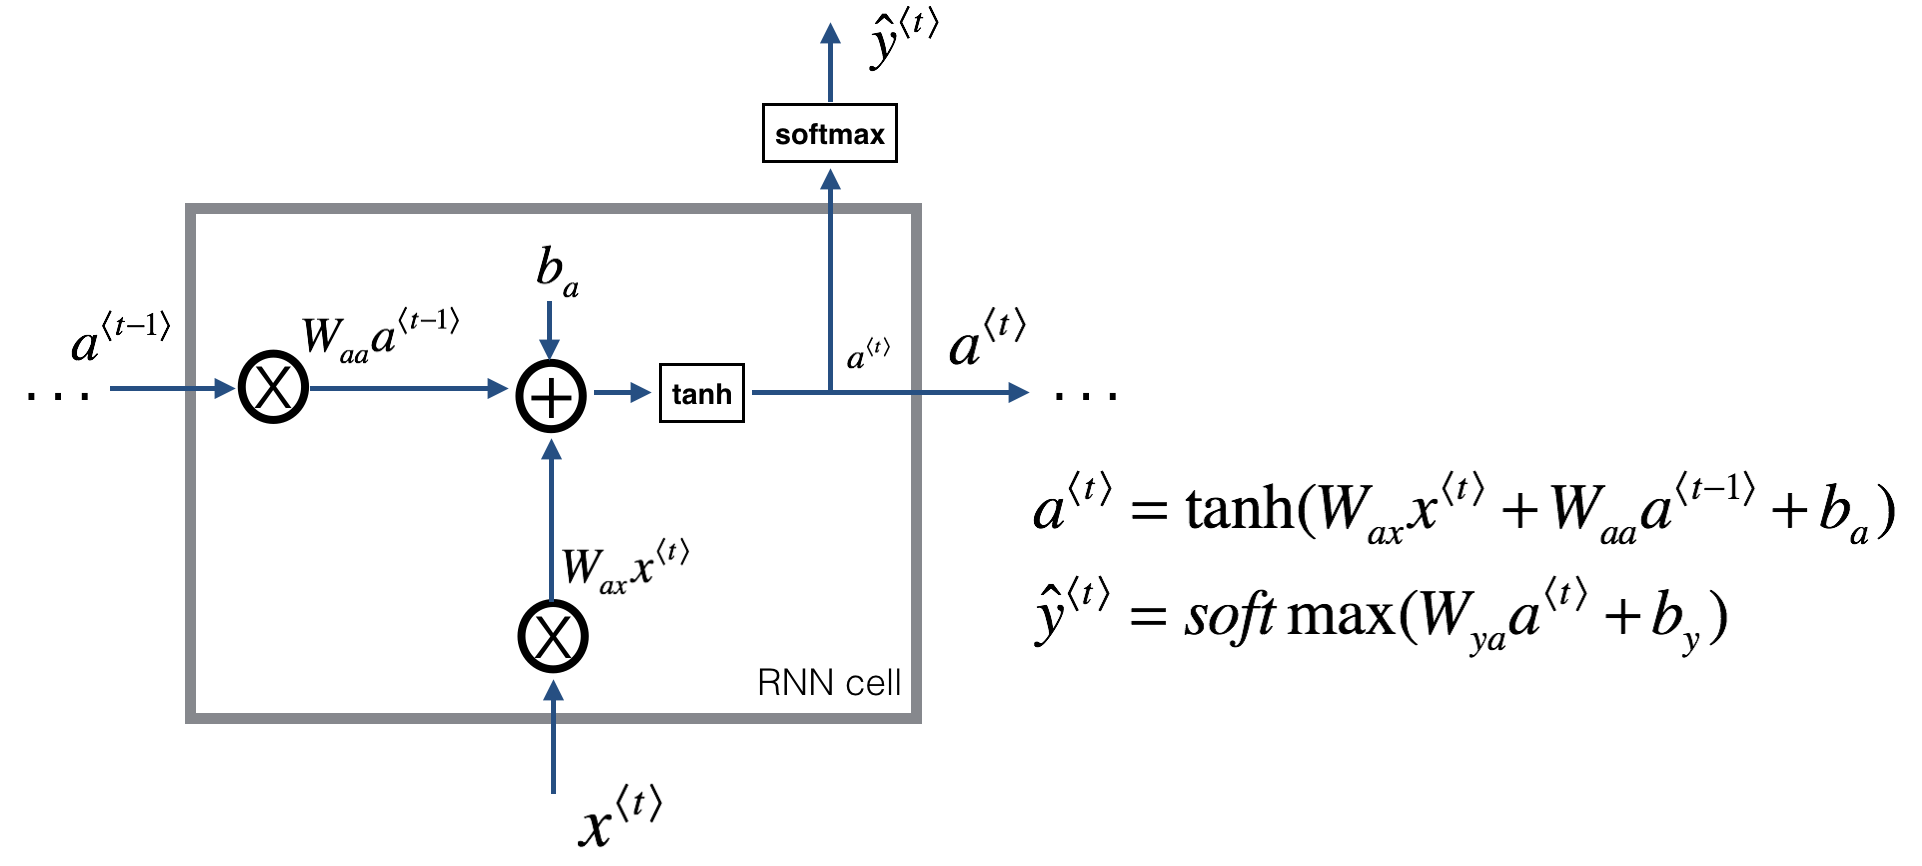
\includegraphics[scale=0.4]{rnn_step_forward.png}
\end{figure}
注意我们的样本总数为$m$,从而$x^{<t>}$的维数为$(n_x,m)$, $a^{t}$的维数为$(n_a,m)$, $W_{ax}$的维数为$(n_a,n_x)$, $W_{aa}$的维数为$(n_a,n_a)$, $W_{ya}$的维数为$(n_y,n_a)$。将上面的单个时间点的RNN模块展开,就可以得到如下的RNN基本表示:
\begin{figure}[htb!]
	\centering
	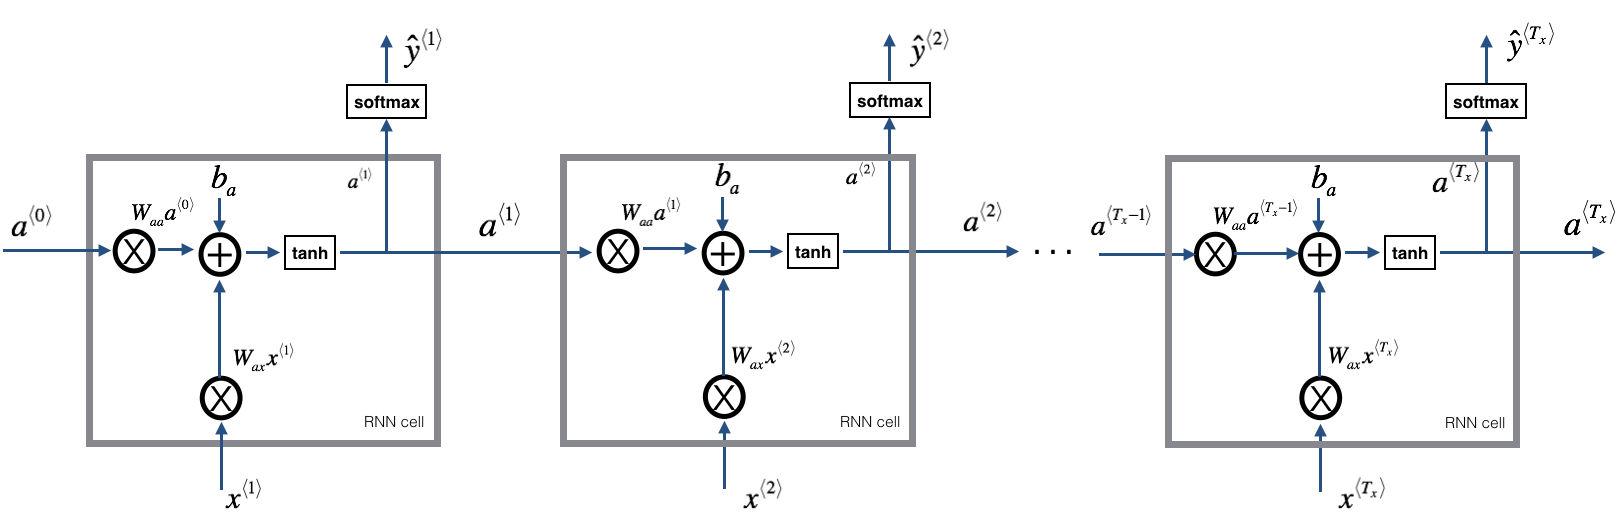
\includegraphics[scale=0.55]{rnn.png}
\end{figure}
\subsection{通过时间的反向传播}
RNN的反向传播过程的大致框架与传统的深度神经网络相同,需要注意的就是网络中的参数$W_a,b_a,W_y,b_y$是共享的。不失一般性,我们定义交叉熵损失作为我们的损失函数,即在单个输出上的损失可以定义为:
\begin{equation*}
\mathcal{L}{(\hat{y}^{<t>},y^{<t>})} = -y^{<t>}\log{\hat{y}^{<t>}}- (1-y^{<t>})\log{(1-\hat{y}^{<t>})}
\end{equation*}
于是损失函数的表达式为:
\begin{equation*}
\mathcal{J} = \sum_{t=1}^{T_y}\mathcal{L}{\left(\hat{y}^{<t>},y^{<t>}\right)}
\end{equation*}
隐藏层的激活函数我们选取$tanh$,于是单个基本块的前向传播过程可以具体写为如下表达式:
\begin{align*}
a^{<t>} &= tanh(W_{ax}x^{<t>}+W_{aa}a^{<t-1>}+b_a)\\
\hat{y}^{<t>} &= soft\max(W_{ya}a^{<t>}+b_y)
\end{align*}
反向传播的数据流图如下所示:
\begin{figure}[htb!]
	\centering
	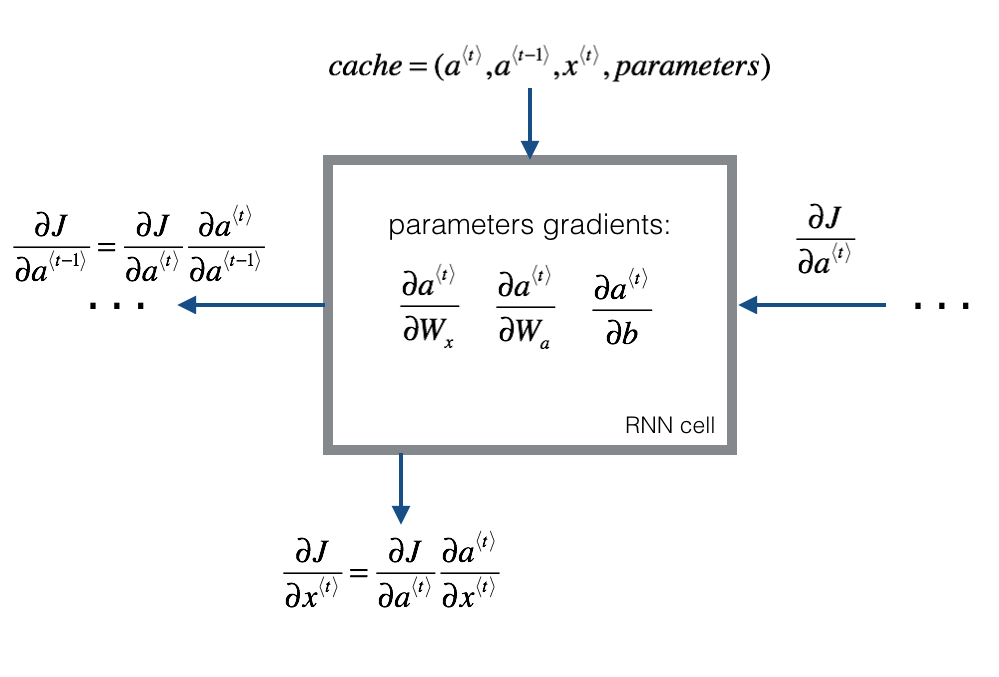
\includegraphics[scale=0.55]{rnn_cell_backprop.png}
\end{figure}


根据上面的数据流示意图,并结合$a^{<t>} = tanh(W_{ax}x^{<t>}+W_{aa}a^{<t-1>}+b_a),\frac{\partial{tanh(x)}}{\partial{x}}=1-tanh(x)^2$,我们可以写出单个RNN模块的反向传播过程的计算公式为:
\begin{align*}
\frac{\partial a^{<t>}}{\partial W_{ax}} &= (1-tanh(W_{ax}x^{<t>}+W_{aa}a^{<t-1>}+b_a)^2)x^{<t>T}\\
\frac{\partial a^{<t>}}{\partial W_{aa}} &= (1-tanh(W_{ax}x^{<t>}+W_{aa}a^{<t-1>}+b_a)^2)a^{<t-1>T}\\
\frac{\partial a^{<t>}}{\partial b_a} &= \sum_{batchsize}(1-tanh(W_{ax}x^{<t>}+W_{aa}a^{<t-1>}+b_a)^2)\\
\frac{\partial{a}^{<t>}}{\partial{x}^{<t>}} &= W_{ax}^T(1-tanh(W_{ax}x^{<t>}+W_{aa}a^{<t-1>}+b_a)^2)\\
\frac{\partial{a}^{<t>}}{\partial{a}^{<t-1>}} &= W_{aa}^T(1-tanh(W_{aa}x^{<t>}+W_{aa}a^{<t-1>}+b_a)^2)
\end{align*}

\end{document}